\chapter{Formatting Text}
\label{formatting}

\section{Emphasis}

Sometimes you need some extra punch to get your point across.
The simplest way to emphasize text in \LaTeX{} is with the \verb|\emph| command,
which \emph{italicizes} its argument by default:
\begin{leftfigure}
\begin{lstlisting}
\emph{Oh my!}
\end{lstlisting}
\end{leftfigure}
gives us
\begin{leftfigure}
\lm \emph{Oh my!}
\end{leftfigure}
There are other tools at our disposal:
\begin{leftfigure}
\begin{lstlisting}
We can use \textbf{boldface} or \textsc{small caps} as well.
\end{lstlisting}
\end{leftfigure}
with
\begin{leftfigure}
\lm%
We can use \textbf{boldface} or \textsc{small caps} as well.
\end{leftfigure}
Be judicious in your use of emphasis, especially boldface.
It excels at drawing the reader's attention away from everything around it,
so too much is distracting.

\section{Meeting the whole (type) family}

The styles shown above are just a few of the many available to you.
A (mostly) complete list follows:
\begin{leftfigure}
\lm
\begin{tabular}{l|l|l}
{\normalfont Command} & {\normalfont Alternative} & {\normalfont Style} \\
\hline
\verb|\textnormal{...}| & \verb|{\normalfont ...}| & the default \\
\verb|\emph{...}| & \verb|{\em ...}| & \emph{emphasis, typically italics} \\
\verb|\textrm{...}| & \verb|{\rmfamily ...}| & roman (serif) type \\
\verb|\textsf{...}| & \verb|{\sffamily ...}| & {\fontspec{Latin Modern Sans}sans serif type} \\
\verb|\texttt{...}| & \verb|{\ttfamily ...}| & {\fontspec[Ligatures=TeX]{Latin Modern Mono}``teletype'' (monospaced)} \\
\verb|\textit{...}| & \verb|{\itshape ...}| & \textit{italics} \\
\verb|\textsl{...}| & \verb|{\slshape ...}| & {\fontspec{Latin Modern Roman Slanted}slanted, or oblique type} \\
\verb|\textsc{...}| & \verb|{\scshape ...}| & \textsc{Small Capitals} \\
\verb|\textbf{...}| & \verb|{\bfseries ...}| & \textbf{boldface} \\
\end{tabular}
\end{leftfigure}
The first form (which takes the text to format as an argument)
should usually be preferred over the second
(which affect the group in which they are issued),
since the former automatically handle any
spacing corrections needed around them.\punckern\footnote{For example,
\textit{italic type} amidst upright type should be followed
by a slight amount of extra space, called an ``italic correction''\quotekern.}
However, there are cases where the second variety is the only option:
\begin{enumerate}
\item When formatting multiple paragraphs. \\
(Command arguments cannot contain paragraph breaks.)
\item When defining the style of other commands.\punckern\footnote{%
For example, this book's section headers are styled with
\texttt{\textbackslash Large\allowbreak\textbackslash itshape}.}

\end{enumerate}

\section{Sizes}

The default text size is controlled by your document class.
It is usually ten points,\punckern\footnote{The standard digital publishing
point, sometimes called the PostScript point, is \otffrac{1}{72} of an inch.
\LaTeX{}, for historical reasons, defines its point (\texttt{pt})
as \otffrac{100}{7227} of an inch
and the former as a ``big point''\quotekern, or \texttt{bp}.}
but this can be adjusted by passing additional arguments to
\verb|\documentclass|.\punckern\footnote{The standard \LaTeX{} classes accept
\texttt{10pt}, \texttt{11pt}, or \texttt{12pt}.
KOMA~Script classes accept arbitrary sizes with
\monobox{fontsize=<size>}.}
To scale text relative to this size, use the following commands:
\begin{leftfigure}
\lm
\renewcommand{\arraystretch}{1.1}
\begin{tabular}{l l}
\verb|\tiny| & \tiny Example Text \\
\verb|\scriptsize| & \scriptsize Example Text \\
\verb|\footnotesize| & \footnotesize Example Text \\
\verb|\small| & \small Example Text \\
\verb|\normalsize| & \normalsize Example Text \\
\verb|\large| & \large Example Text \\
\verb|\Large| & \Large Example Text \\
\verb|\LARGE| & \LARGE Example Text \\
\verb|\huge| & \huge Example Text \\
\verb|\Huge| & \Huge Example Text \\
\end{tabular}
\end{leftfigure}
There are some subtleties at play here.
\LaTeX's default type family, Latin Modern,
comes in multiple \introduce{optical sizes}.
Smaller fonts aren't just shrunken versions of their big siblings---they
have thicker strokes, exaggerated features,
and more generous spacing to improve legibility at their size.
\begin{leftfigure}
\fontspec{lmroman5-regular} If you magnify 5 point type
\fontspec{lmroman10-regular} and place the result next to 11 point type,
the differences are immediately noticeable.
\end{leftfigure}
In the days of metal type, optical sizes were standard, but
many digital typefaces lack them,
given how much more work it demands from the type
designer.\punckern\footnote{If you are fortunate enough to have
a typeface with multiple optical sizes, \XeLaTeX{}
and \LuaLaTeX{} can make good use of them! See \chapref{fonts}
for more on font selection and OpenType features.}

But points and optical sizes don't tell the whole story.
Each typeface has its own proportions, which make a huge difference
in perceived size.
(Compare Garamond, {\fontspec{Latin Modern Roman} Latin Modern},
and {\fontspec{NHaasGroteskTXPro-55RG}Helvetica}, all at 11\,pt.)
Shown below are some common terms:
\begin{centerfigure}
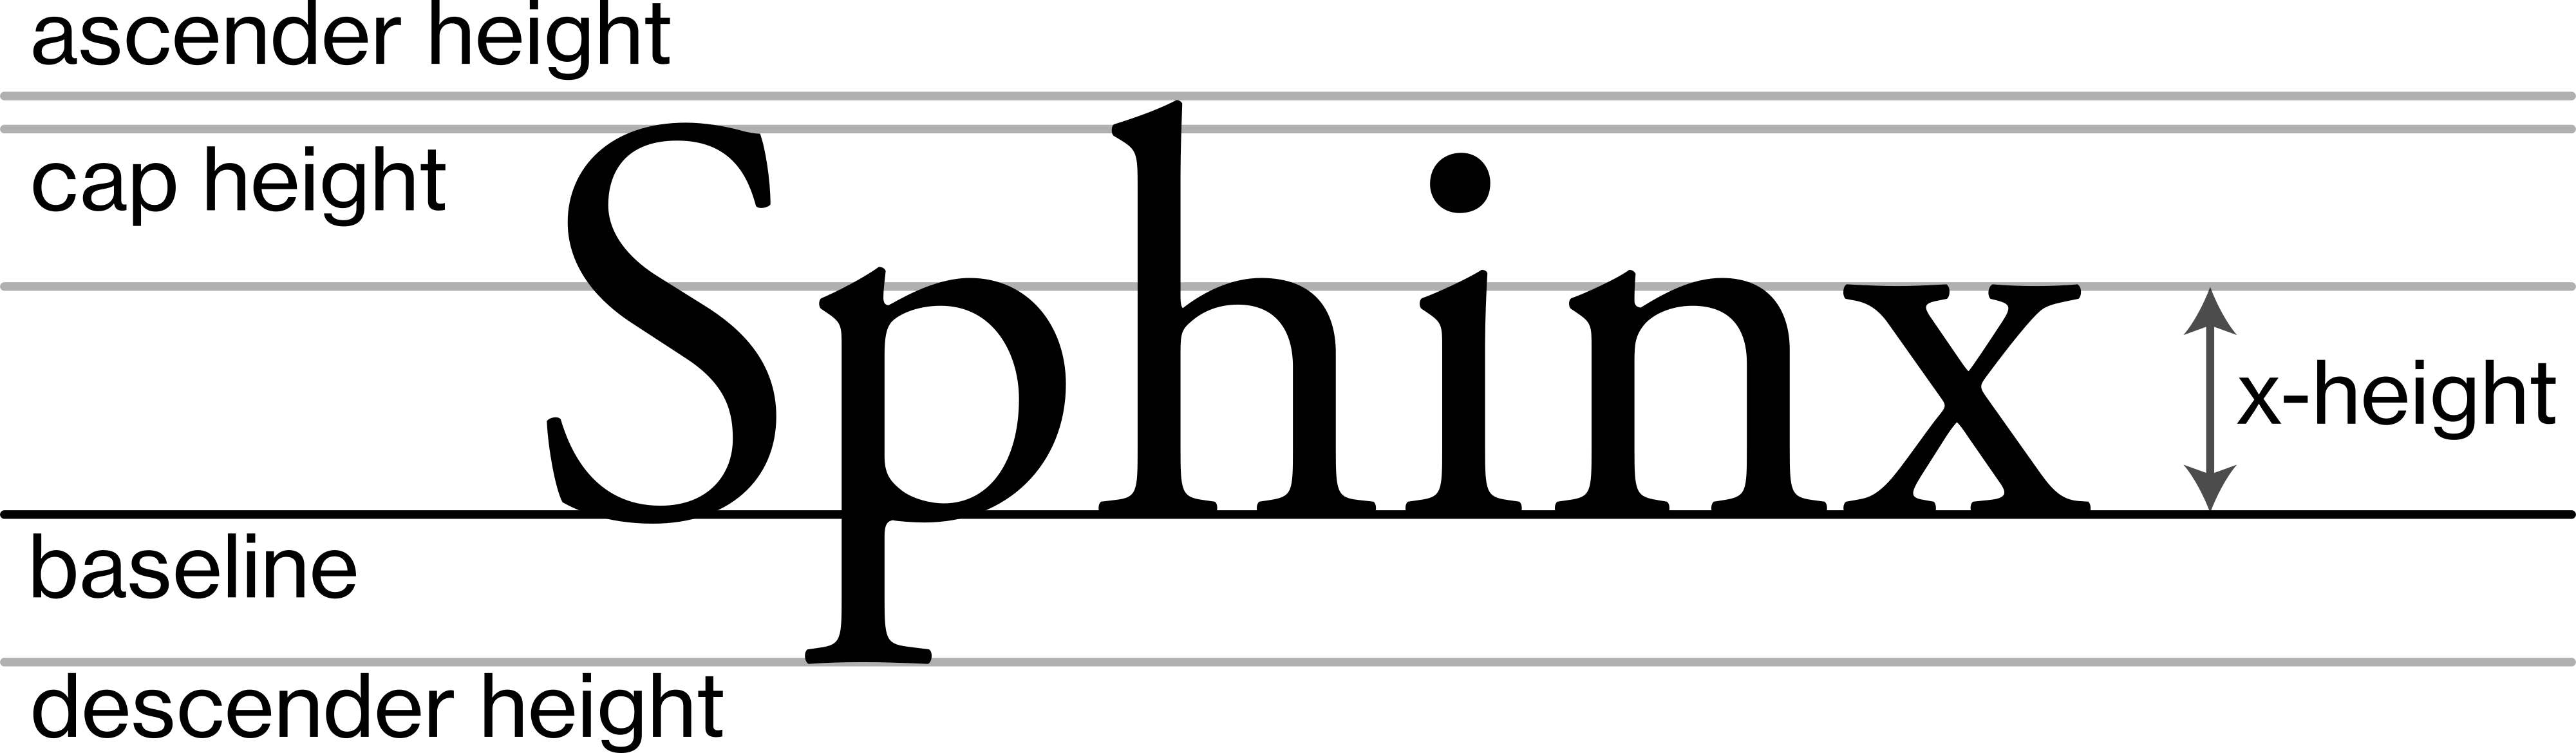
\includegraphics[keepaspectratio,width=0.65\textwidth]{heights.png}

\captionof{figure}{Type sits on the \introduce{baseline},
rises to the \introduce{ascender height},
and drops to the \introduce{descender height}.
The \introduce{cap height} refers to the size of uppercase letters,
and the \introduce{x-height} refers to the size of lowercase letters.}
% For size reference:
%{\sffamily\fontsize{8pt}{8pt}\selectfont This is 8-point text.}
\end{centerfigure}

If the previous commands aren't enough, you can create custom sizes with
\verb|\fontsize|, which takes both the desired point size and the
distance between baselines.
This must be followed with \verb|\selectfont| to take effect.
For example, \texttt{\textbackslash fontsize\{30pt\}\allowbreak\{30pt\}%
\allowbreak\textbackslash selectfont}
gives:
\begin{leftfigure}
\lm
\fontsize{30pt}{30pt}\selectfont
large type with no extra \\
space between lines
\end{leftfigure}
{\fontsize{10pt}{10pt}\selectfont
Note that without extra spacing,
or \introduce{leading},\punckern\footnote{This term comes from the days of
metal type, when strips of lead were inserted
between lines to give them extra spacing.}
descenders from one line nearly collide with ascenders and capitals on
the line below.
Leading is important---without it, blocks of text become uncomfortable to
read, especially at normal body sizes.\par}
Let your type breathe.\punckern\footnote{For a discussion on optimal leading,
see \textit{Practical Typography}, listed in Appendix~\ref{resources}.}

\section{What next?}
\begin{itemize}
\item Learn how to underline text using the \texttt{ulem}
    package.\punckern\footnote{Other typographical tools---like italics,
    boldface, and small caps---are generally preferable to underlining,
    but it has its uses.}
\item Use KOMA~Script to change the size and style of your section headings.
\item Learn the difference between italic and oblique type.
\end{itemize}
